\subsection{Election November 3, 1896: *McKinley vs Bryan}
\begin{frame}[t]{Election November 3, 1896: *William McKinley}
\small
% Lincoln
\begin{columns}[T, onlytextwidth]
\column{0.48\textwidth}
\vspace{-1em}
{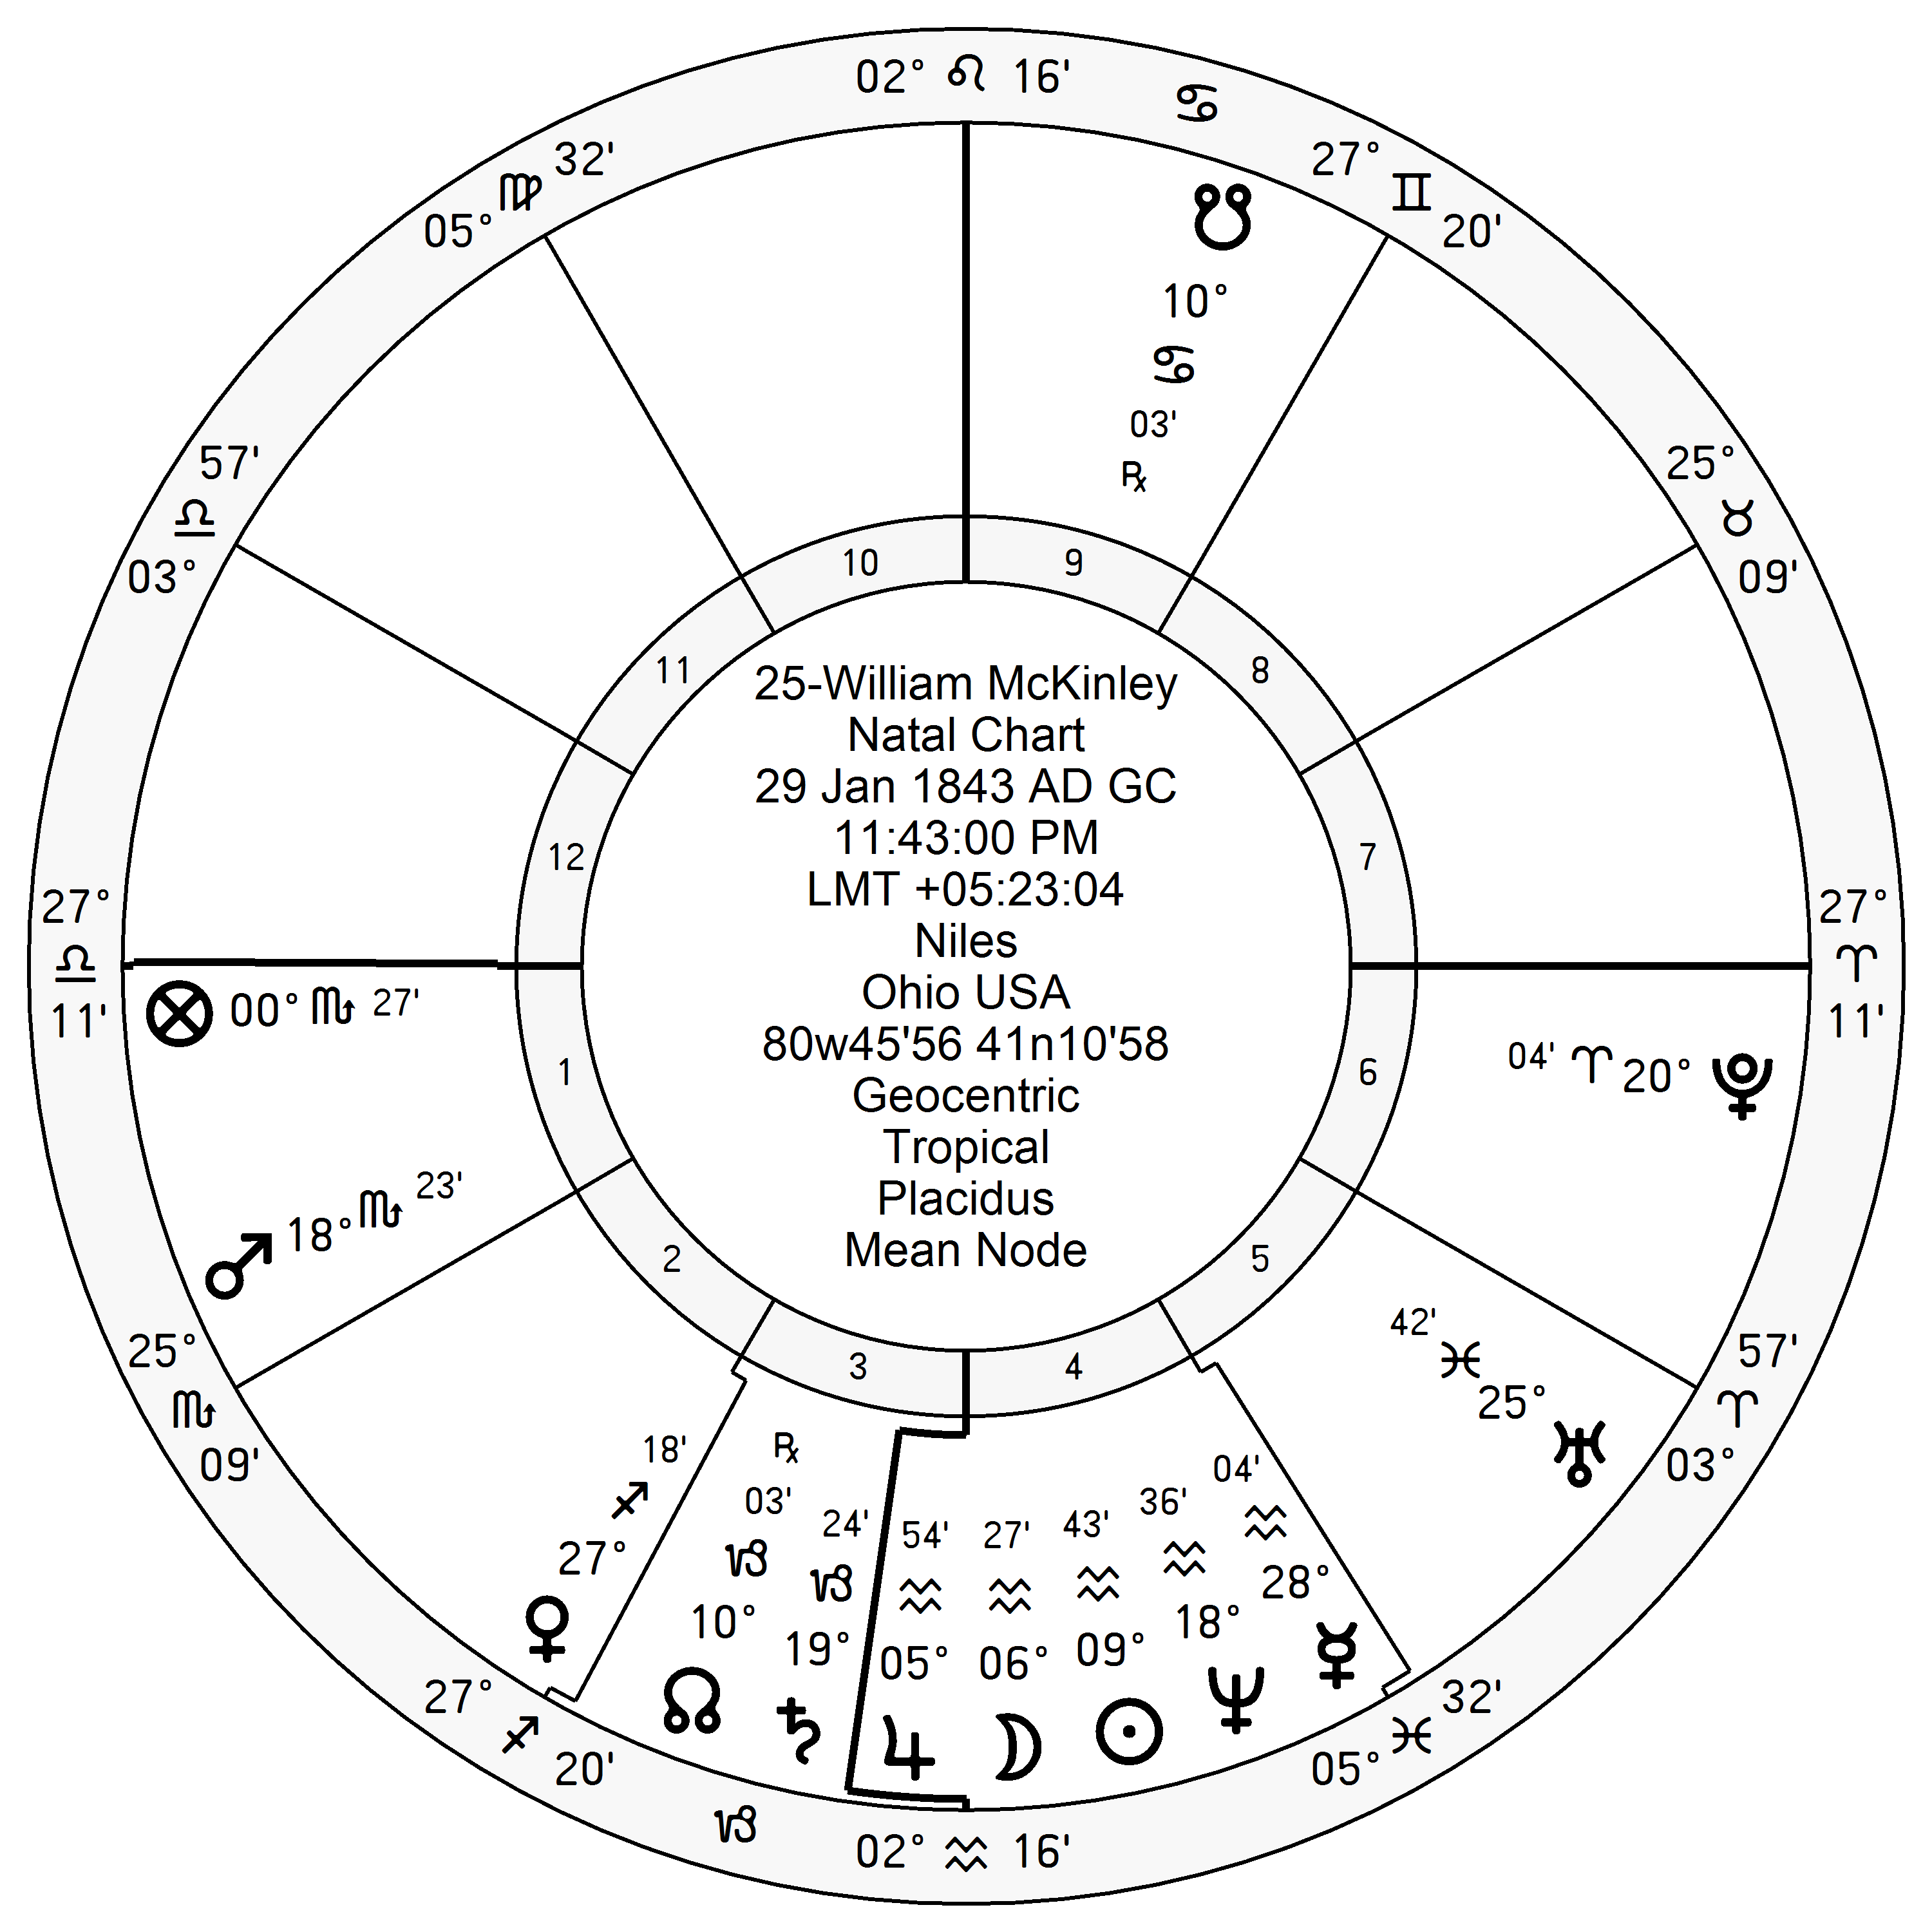
\includegraphics[width=0.9\textwidth]{charts/McKinley.png}}
\fontsize{8pt}{9pt}\selectfont

\Jupiter\, \Sextile\, P1, \Square\, N1, \Opposition\, N10. Disposited by \Saturn\, in domicile in P10.

\column{0.48\textwidth}
\vspace{-1em}
{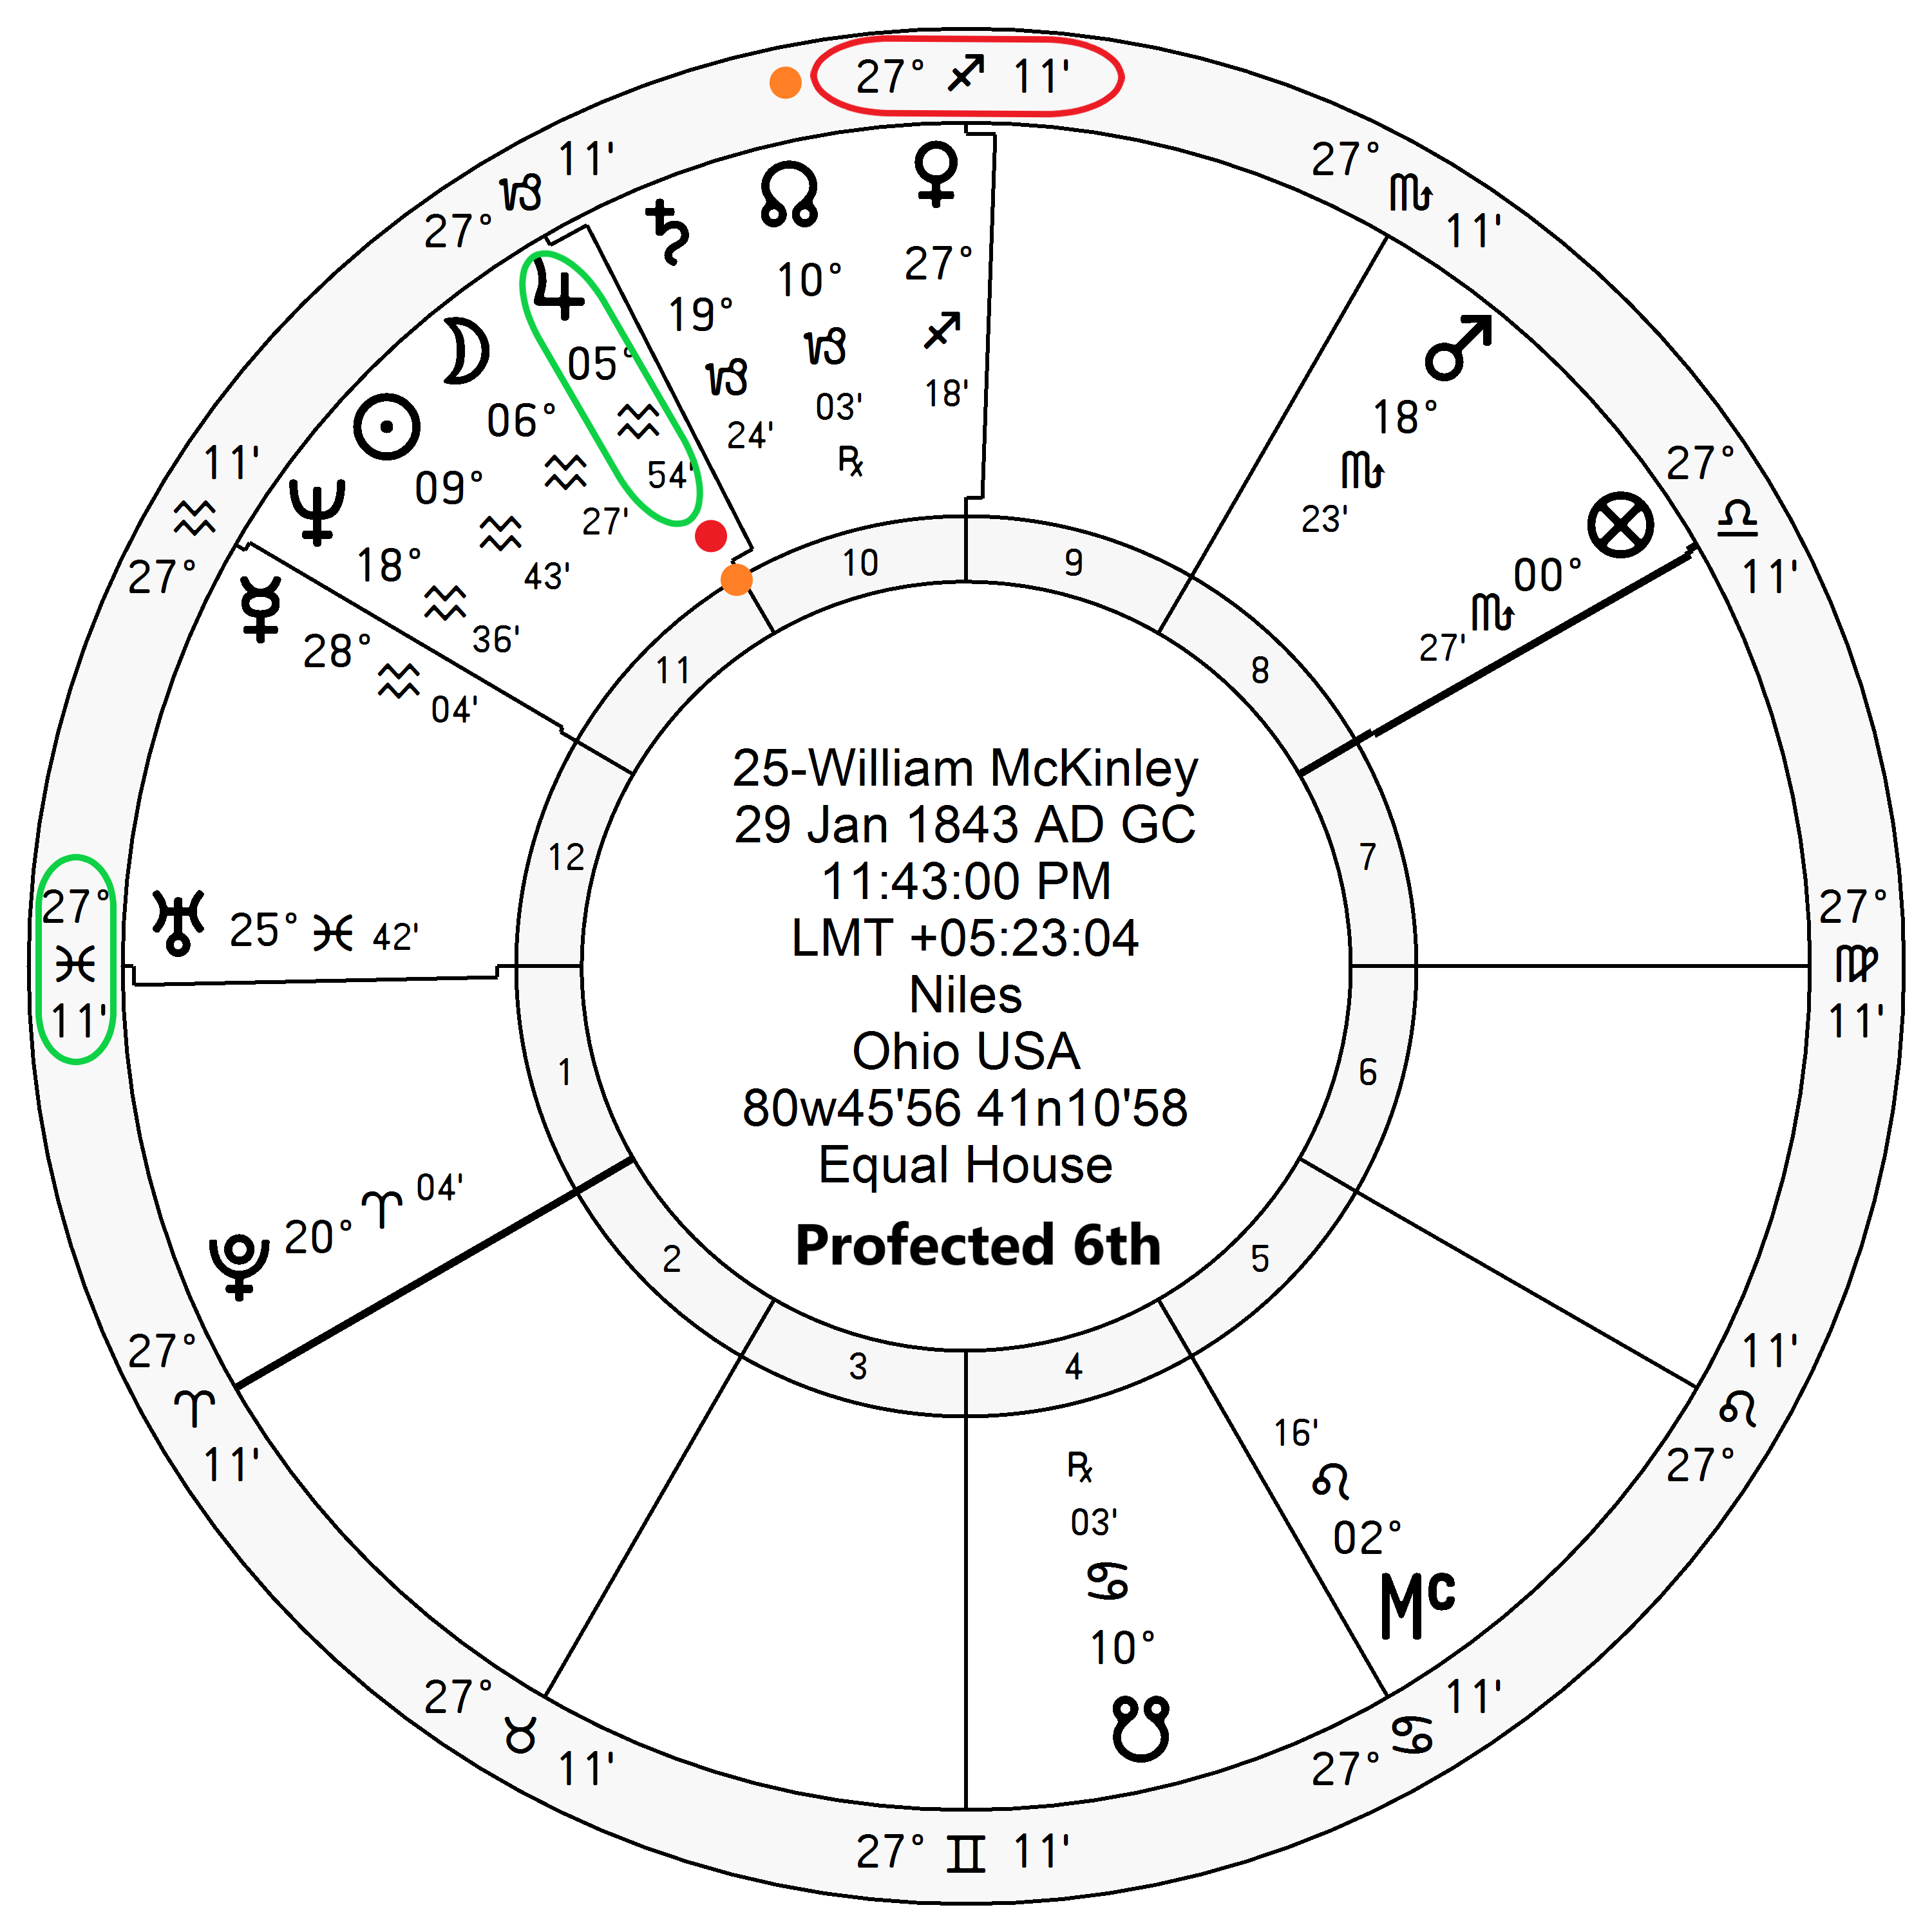
\includegraphics[width=0.9\textwidth]{charts/McKinley-Prof-6th.png}}
\textbf{\dgreen P1}=N5 
	$\Rightarrow$ \Jupiter\, $\Rightarrow$ \textbf{\dgreen P11/N4} \\
\textbf{\red P10=N3} 
	$\Rightarrow$  \Jupiter\, $\Rightarrow$  \textbf{\dgreen P11/N4} \\
PE=\textbf{\red P10/N3} 
	$\Rightarrow$  \Jupiter\, $\Rightarrow$  \textbf{\dgreen{P11/N4}}

\end{columns}
\end{frame}

% McClellan
\begin{frame}[t]{Election November 3, 1896: William Jennings Bryan}
\small
\begin{columns}[T, onlytextwidth]
\column{0.48\textwidth}
\vspace{-1em}
{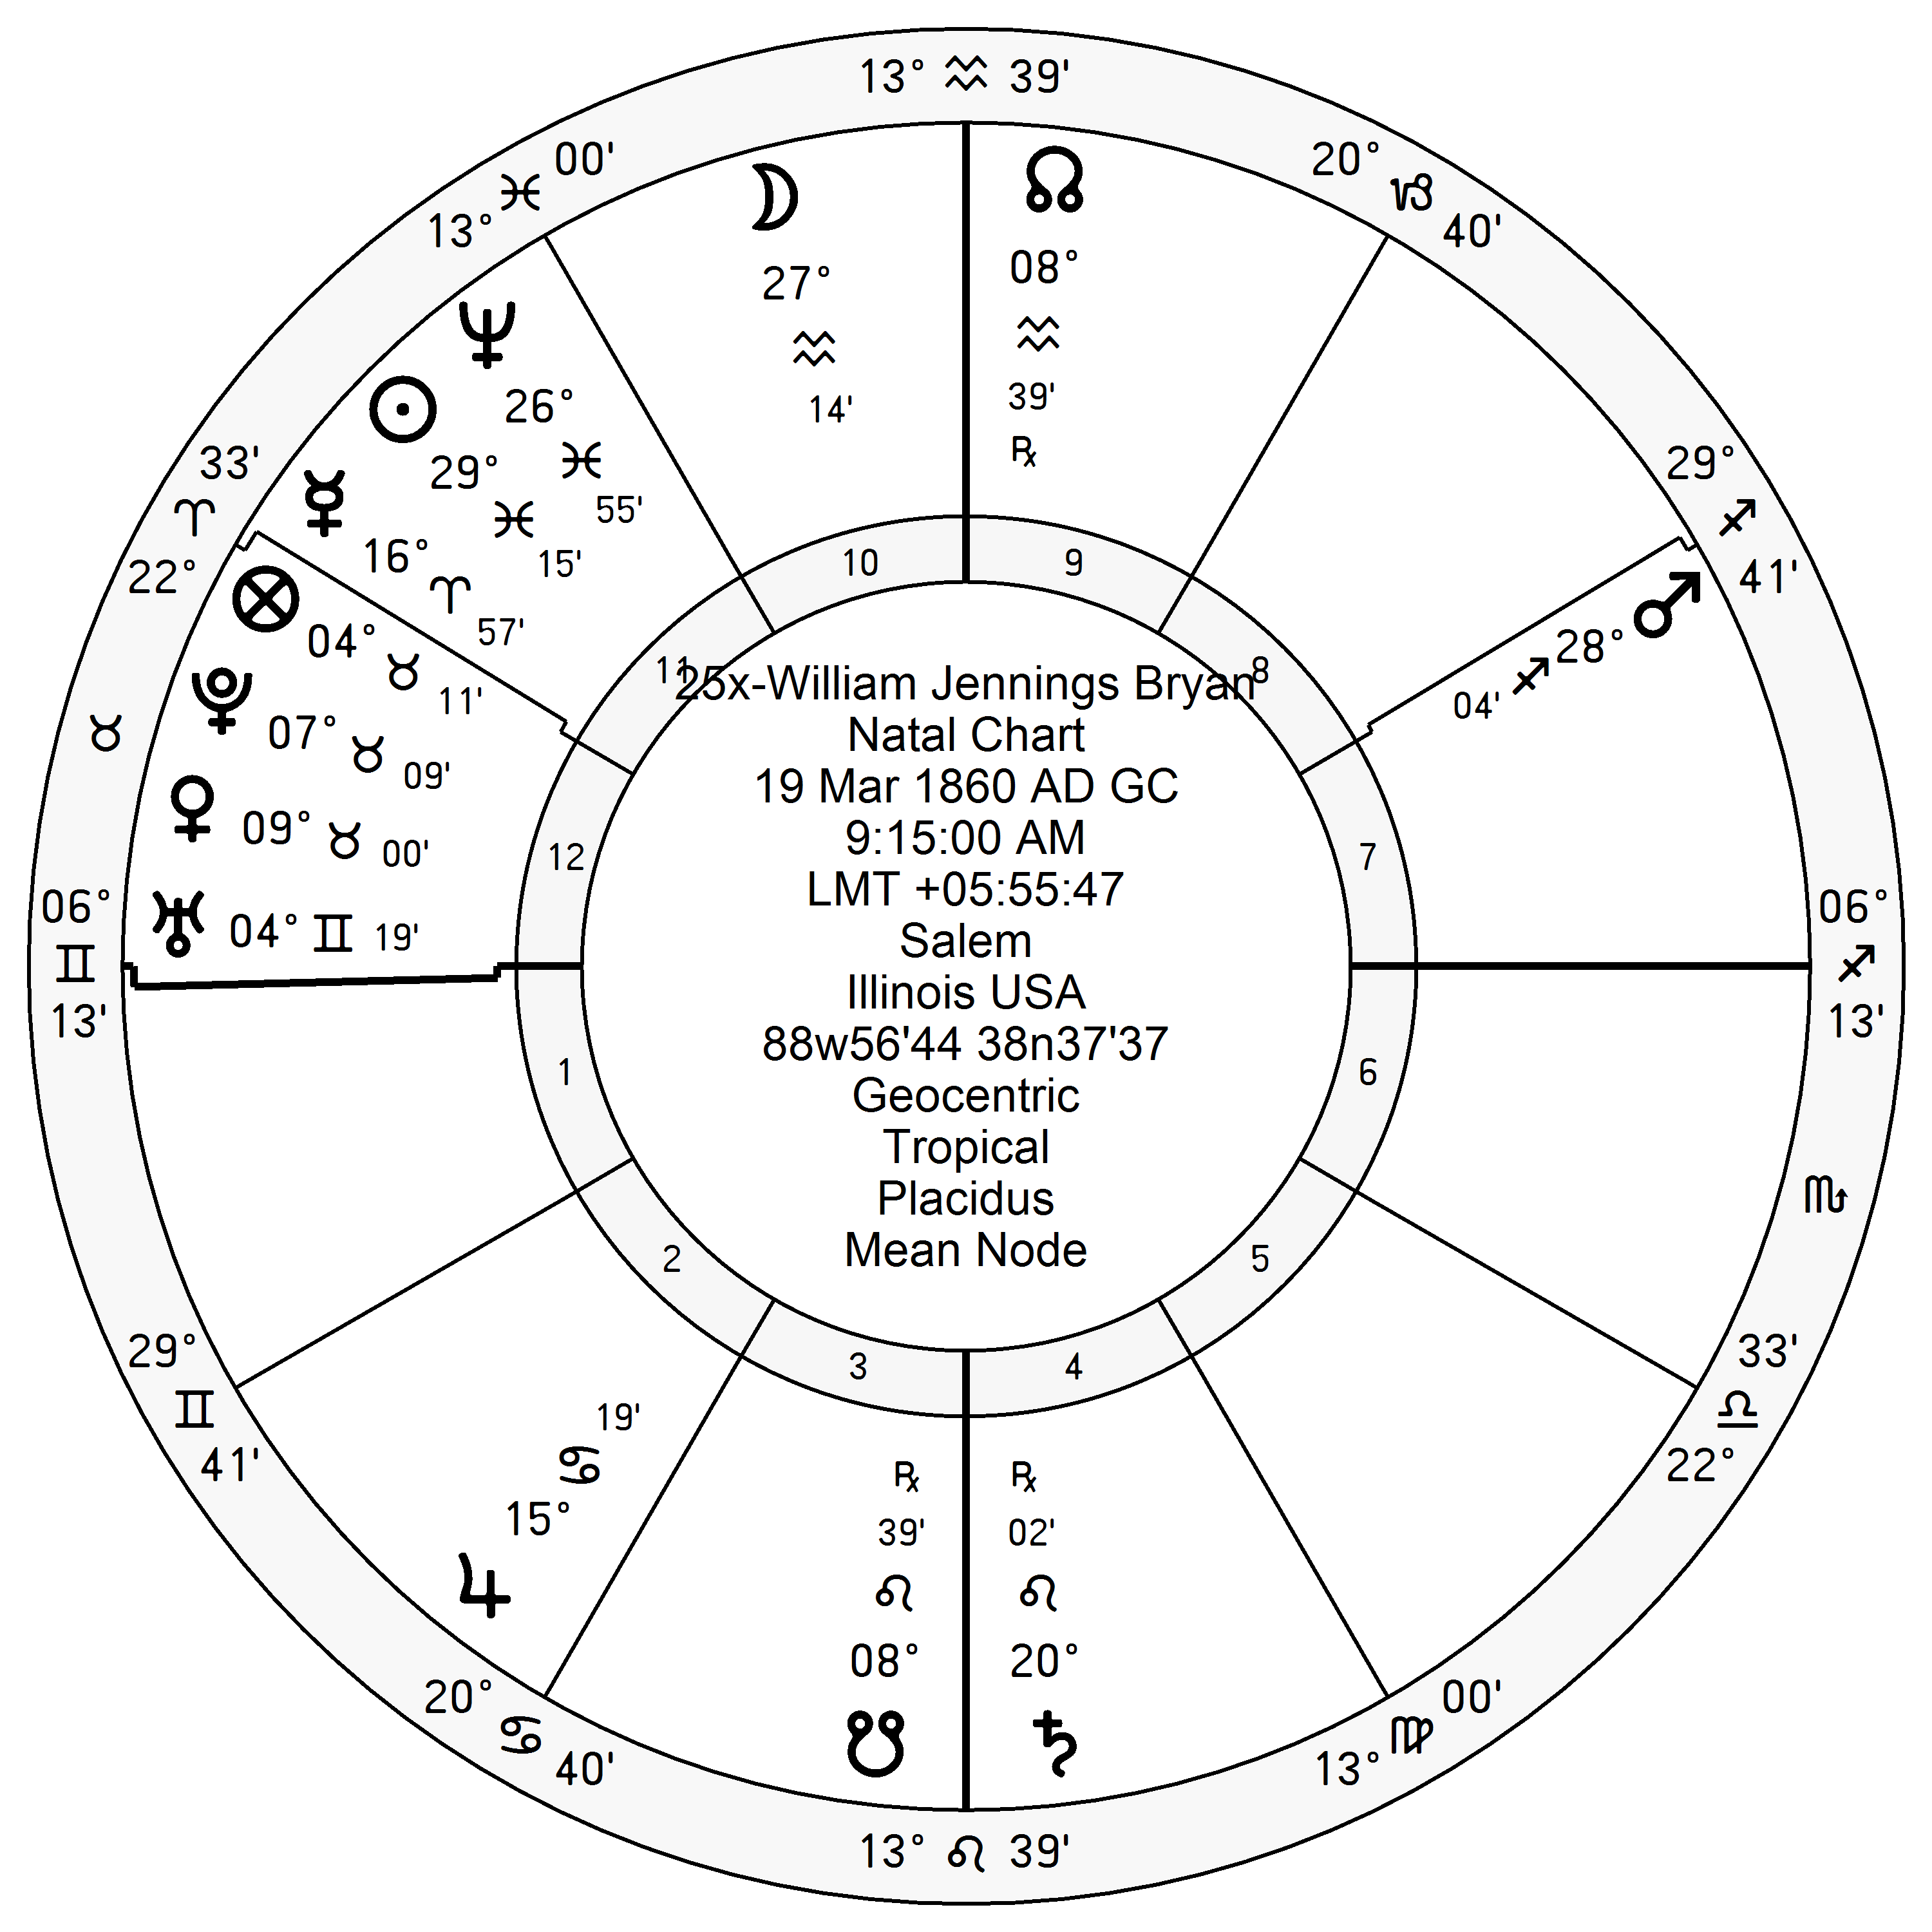
\includegraphics[width=0.9\textwidth]{charts/Bryan.png}}
\fontsize{8pt}{9pt}\selectfont

\Mercury\, is \Sextile\, N10; \Sextile\, P1. \\
\Jupiter\, \Trine\, P10, N10. \\
\Saturn\, averse to P10, \Opposition\, N10; \Sextile\, P1, N1. \\
In the profection, \Saturn\, and the \SouthNode\, are in the same sign and house; the South Node tends to be destructive.

\column{0.48\textwidth}
\vspace{-1em}
{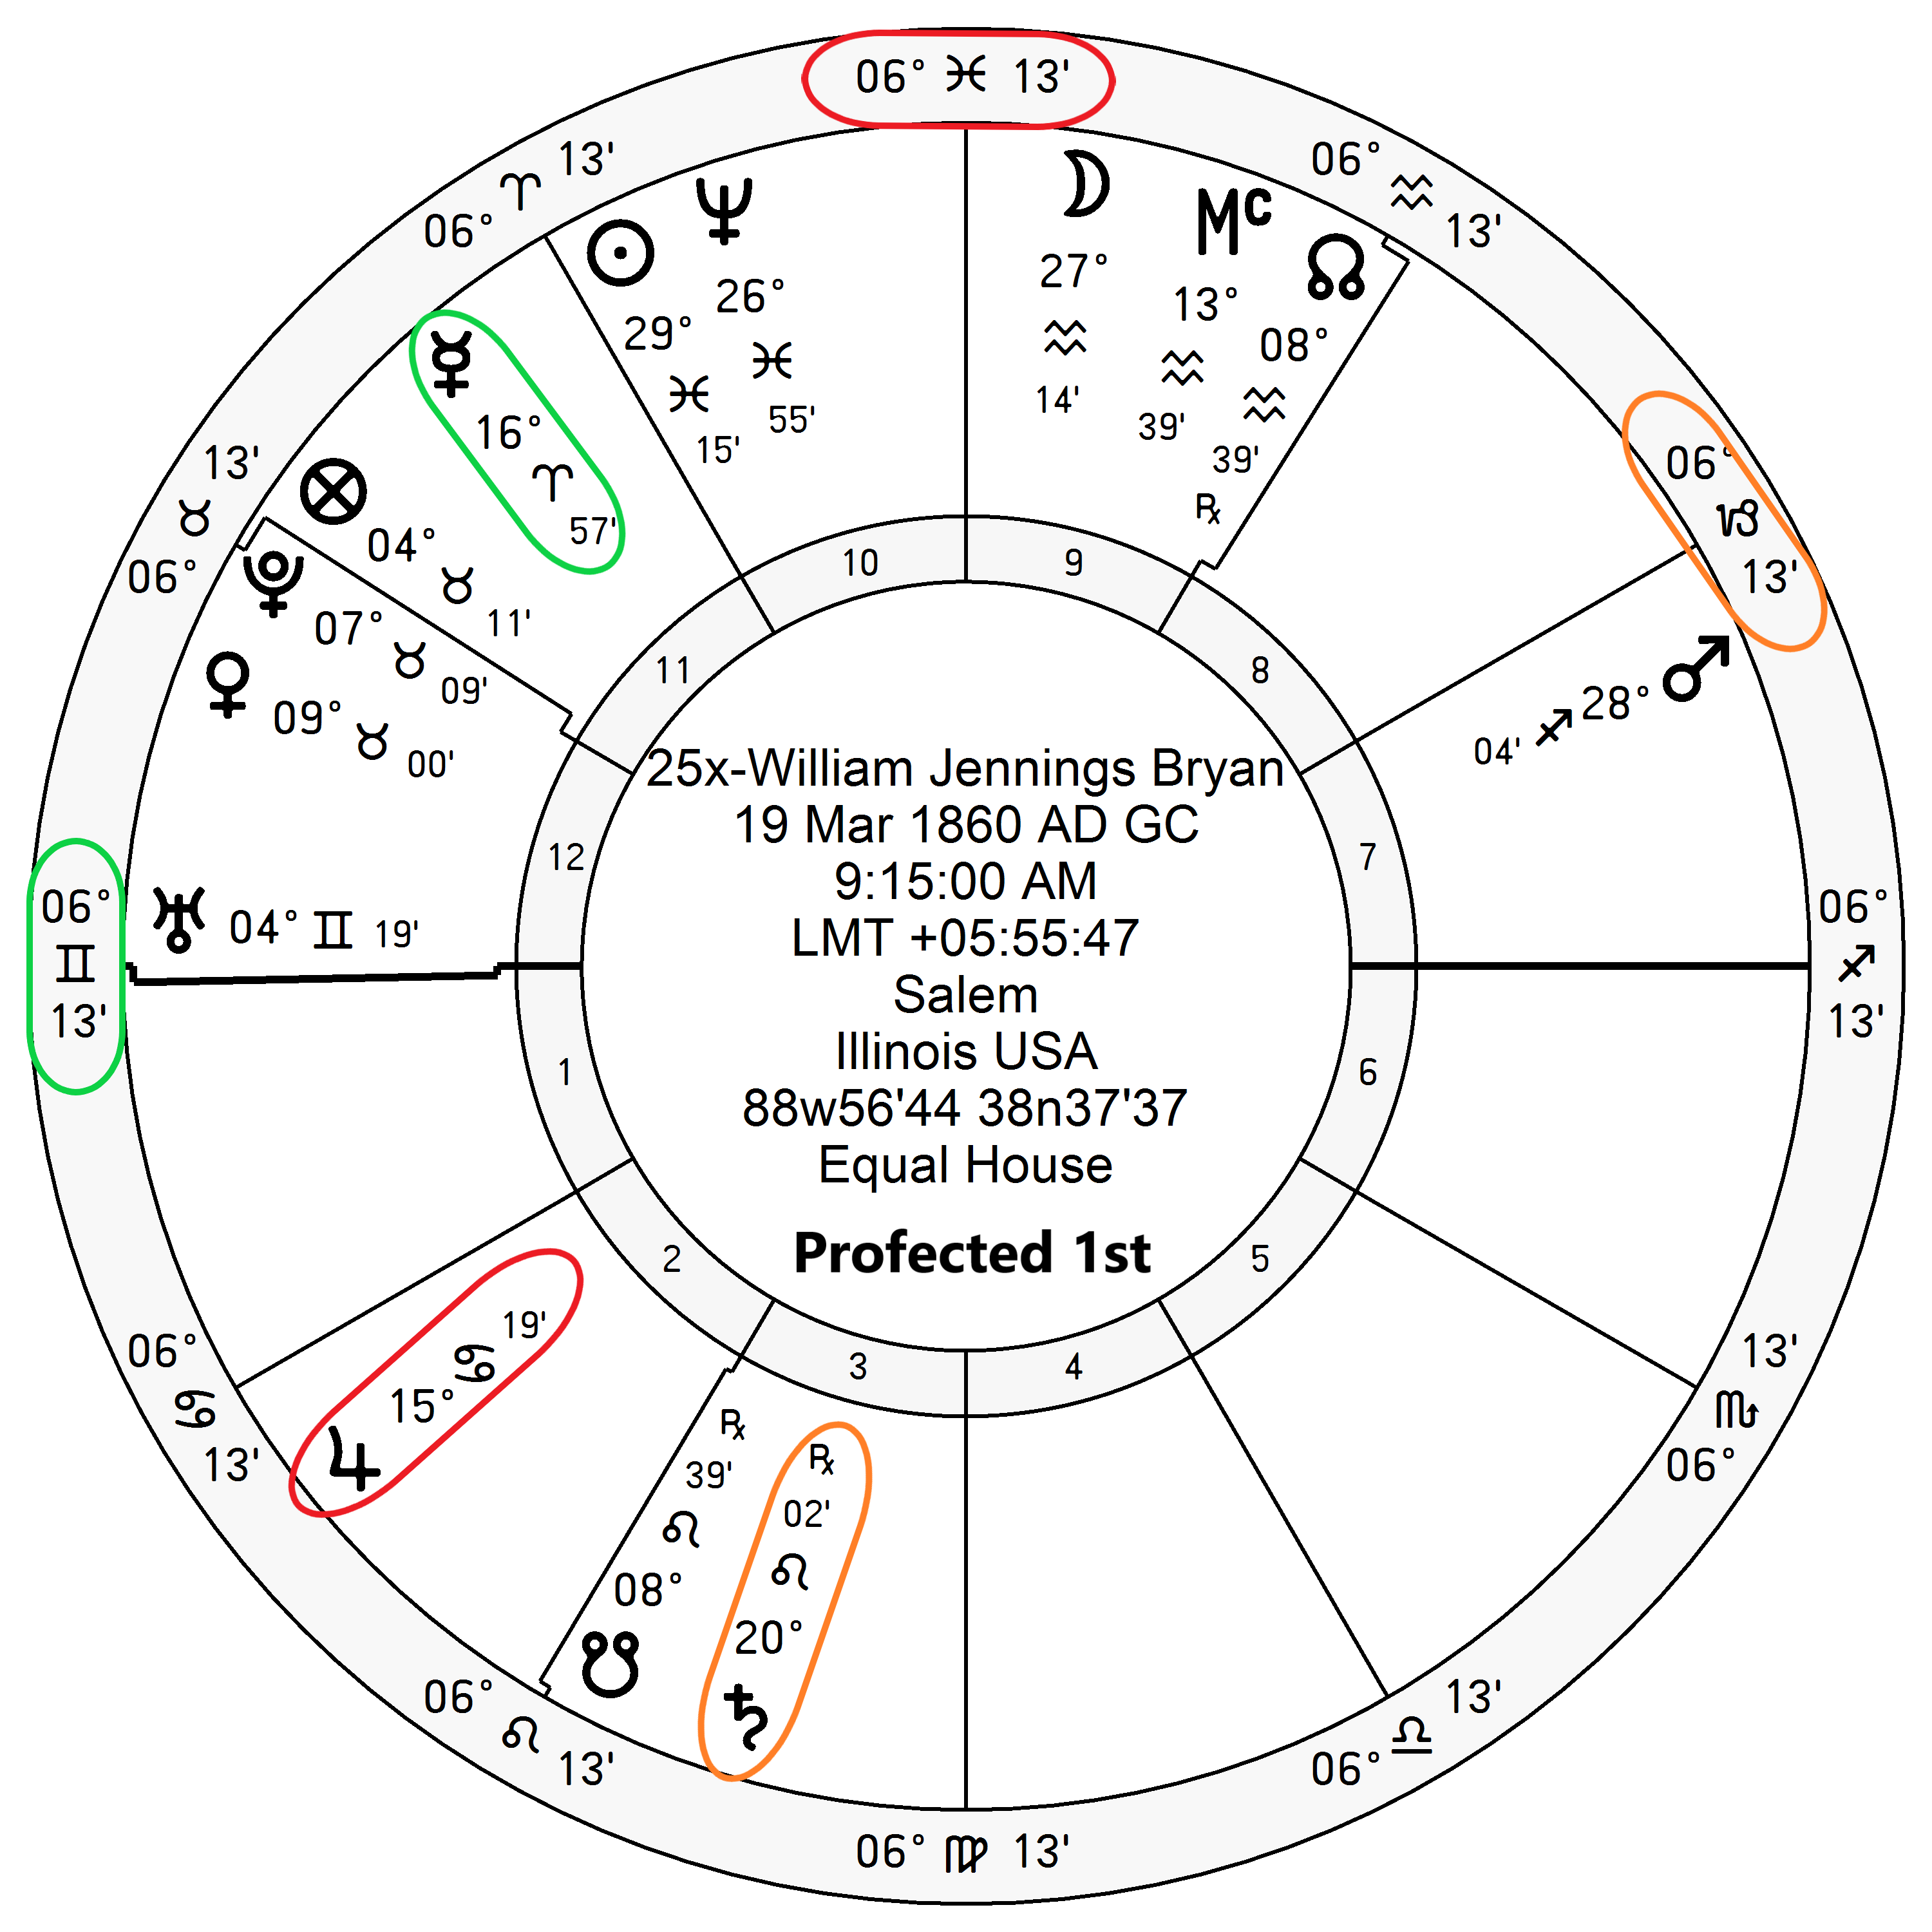
\includegraphics[width=0.9\textwidth]{charts/Bryan-Prof-1st.png}}
\textbf{\dgreen P1=N1} 
	$\Rightarrow$ \Mercury\, $\Rightarrow$ P11/N11\\
\textbf{\red P10=N10}
	$\Rightarrow$ \Jupiter\, $\Rightarrow$ P2/N2\\
PE=P8/N8 
	$\Rightarrow$ \Saturn\,\Retrograde $\Rightarrow$ P3/N4
\end{columns}
\end{frame}
